\section{Конденсаторы}

Конденсатор --- \hrulefill

\hrulefill

\hrulefill

Обозначение конденсатора в схеме:

\begin{tikzpicture}
\draw (0,0) rectangle (6,2);
\end{tikzpicture}

Единицы измерения емкости конденсатора:

\begin{tikzpicture}
\draw (0,0) rectangle (6,2);
\end{tikzpicture}

\subsection{Плоский конденсатор}

Плоский конденсатор --- \hrulefill

\hrulefill

\hrulefill

Емкость плоского конденсатора:

\begin{tikzpicture}
\draw (0,0) rectangle (6,2);
\end{tikzpicture}

\subsubsection{Устройство плоского конденсатора}

\begin{figure}[h]
\centering
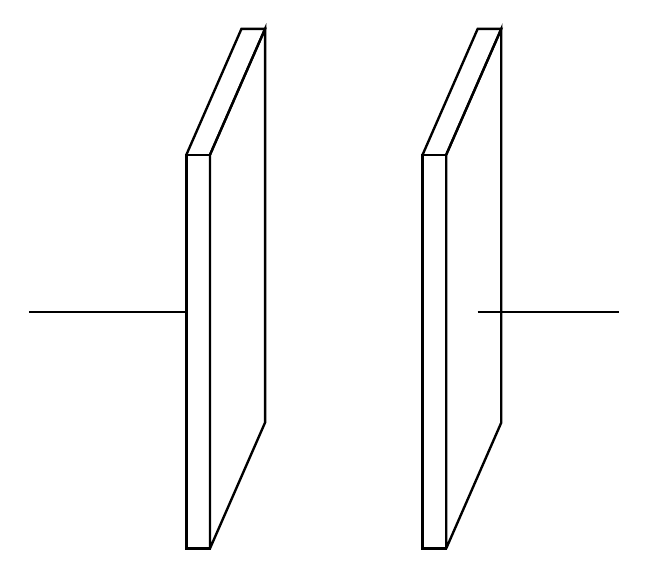
\begin{tikzpicture}
%левая обкладка
\draw[line width = 0.3mm](0,0) rectangle (0.3,5);
\draw[line width = 0.3mm] (0.3,0) --  (1,1.6) -- (1,6.6) -- (0.3,5) -- (0.3,0); 
\draw[line width = 0.3mm]  (0,5) -- (0.7,6.6) -- (1,6.6) -- (0.3,5);


%правая обкладка
\draw[line width = 0.3mm](3,0) rectangle (3.3,5);
\draw[line width = 0.3mm] (3.3,0) --  (4,1.6) -- (4,6.6) -- (3.3,5) -- (3.3,0); 
\draw[line width = 0.3mm]  (3,5) -- (3.7,6.6) -- (4,6.6) -- (3.3,5);

\draw[line width = 0.3mm] (-2,3) -- (0,3);

\draw[line width = 0.3mm] (3.7,3) -- (5.5,3);


\end{tikzpicture}
\caption{Устройство конденсатора}
\label{fig:capacitor}
\end{figure}


\subsection{Время зарядки конденсатора}
Чтобы узнать, за какое время конденсатор заряжается и разряжается, используется одна интересная зависимость.
Рассмотрим новую величину, описывающую время заряда конденсатора --- постоянная времени. Эта величина обозначается буквой $\tau$ (тау), и равна она:

\begin{tikzpicture}
\draw (0,0) rectangle (6,2);
\end{tikzpicture}

%$$\tau = RC$$
Ее значение описывает время, за которое конденсатор зарядится на $\ \sim \! 33.3\%$.
\\
Данная постоянная зависит \hrulefill

\hrulefill
%только от величины и параметров резистора и конденсатора, но не зависит от величины тока, протекающего в цепи, и напряжения на элементах. Ее зависимость выводится из дифференциального уравнения. 
\\
Из эмпирических данных известно, чтобы зарядить или разрядить конденсатор на $99\%$, что обычно достаточно для прикладных задач, то время $t$ будет равно \hrulefill.

% $t = 5\tau = 5RC$.
%Рассмотрим цепь:

%\begin{figure}[h]
%\centering
%\begin{circuitikz}
%\draw (0,0) to[R, l=R] (4,0) -- (4,2) to[C, l = C](0,2) --(0,0);
%\end{circuitikz}
%\caption{Заряд и разряд конденсатора}
%\label{fig:cap}
%\end{figure}
%
%Значение тока заряда в этой цепи будет равно:
%$$I = C \frac{dU}{dt},$$
%\\
%при этом сила тока на резисторе из закона Ома равняется:
%\\
%$$I = \frac{U}{R},$$
%\\
%где $U$ --- напряжение на конденсаторе.
%\\
%Из первого правила Кирхгофа можно записать следующее выражение:
%\\
%$$\frac{U}{R} = - C \frac{dU}{dt},$$
%\\
%Это обычное дифференциальное уравнение с раздедяющимися переменными. Все с $U$ в одну сторону, с $t$ в другую:
%\\
%$$\frac{dU}{U} = - \frac{dt}{RC},$$
%\\
%возьмем интеграл:
%\\
%$$ \int \frac{dU}{U} = - \int \frac{dt}{RC},$$
%\\
%В итоге получаем:
%\\
%$$\ln U = -\frac{t}{RC} + Const,$$
%\\
%$$U = e^{-\frac{t}{RC}} \cdot e^{Const}.$$
%\\
%Эта формула выражает зависимость в цепи напряжения $U$ от времени $t$, а произведение $RC$ обозначается одной буквой $\tau$, тем самым получаем постоянную времени, и можем переписать уравнение:
%\\
%$$U = e^{-\frac{t}{\tau}} \cdot e^{Const}$$.
%\\
%Эта зависимость является экспоненциальной, поэтому график разряда выглядят вот так:
%\begin{center}
%\begin{tikzpicture}
%\begin{axis}[xlabel = {$t$}, xmin = 0, xmax=10]
%\addplot[blue] {exp(-x)};
%\end{axis}
%\end{tikzpicture}
%\end{center}



\subsection{Сопротивления конденсатора}

\begin{enumerate}
	\item Соберите схему, представленную на рисунке \ref{ris:8.1}.  Убедитесь в том, что лампа горит. 
	\item Соберите схему \ref{ris:8.1}, представленную на рисунке. Конденсатор в этом случае включен в цепь постоянного тока. Убедитесь в том, что лампа не горит. 
	\item Сделайте вывод о сопротивлении конденсатора, включенного в цепь постоянного тока.
\end{enumerate}

\begin{figure}[h]
\begin{minipage}[h]{0.5\linewidth}
\center{\begin{circuitikz}[european] \draw
(0,0) to[battery, invert] (0,2) -- (4,2)  to[lamp] (4,0) -- (0,0)
 ;
\end{circuitikz}}
\end{minipage}
\hfill
\begin{minipage}[h]{0.5\linewidth}
\center{\begin{circuitikz} \draw
(0,0) to[battery, invert] (0,2) to[ecapacitor] (4,2)  to[lamp] (4,0) -- (0,0)
;
\end{circuitikz}}
\end{minipage}
\caption{Сопротивление конденсатора}
\label{ris:8.1}
\end{figure}

Вывод --- \hrulefill

\hrulefill

\hrulefill


\subsection{Зарядка и разрядка конденсатора}

\begin{enumerate}
	\item Соберите схему, представленную на рисунке \ref{fig:8.2}. Укажите направление силы тока в ней при зарядке и разрядке конденсатора.
	\item Зажмите кнопку $K_1$. Засеките время заряда конденсатора по яркости светодиода и по показаниям вольтметра. Результаты измерений занесите в таблицу \ref{tab:8.2}. 
	\item Отпустите кнопку $K_1$ и замкните выключатель $K_2$. Засеките время разрядки конденсатора по показаниям вольтметра. Результаты измерений занесите в таблицу \ref{tab:8.2}.
	\item Рассчитайте для каждого случая постоянную времени $\tau$, и занесите ее в таблицу \ref{tab:8.2}.
	\item Запишите вывод о времени зарядки и разрядки конденсаторов разной емкости. 
\end{enumerate}

\begin{figure}[h]
    \centering
    \begin{circuitikz}
        \draw(0,0) -- (0,1) to[battery1, invert] (0,1.5) to[battery1, invert, l=$\mathscr{E}$] (0,2) to[battery1, invert] (0,2.5) to[battery1, invert] (0,3) -- (0,4);
        \draw (0,4) to[empty led, l=$\text{Кр}$, fill=red] (2,4) to[R, l=$R_1$] (4,4) -- (6,4) to[normal open switch, l=$K_2$](8,4);
        \draw (8,4) to[R, l=$R_2$] (8,0)  -- (3,0) to[push button, l=$K_1$, mirror] (0,0);
        \draw (4,4) to[rmeter, t=$V$](4,0);
        \draw (6,4) to[ecapacitor, l=C](6,0);
    \end{circuitikz}
    \caption{Зарядка и разрядка конденсатора}
    \label{fig:8.2}
\end{figure}


\begin{table}[h]
\caption{Зарядка и разрядка конденсатора}
\label{tab:8.2}
\begin{tabular}{|c|cc|c|c|cc|cc|}
\hline
\multirow{2}{*}{№} & \multicolumn{2}{c|}{Сопротивление}           & \multirow{2}{*}{\begin{tabular}[c]{@{}c@{}}Электроемкость \\ С, мкФ\end{tabular}} & \multirow{2}{*}{\begin{tabular}[c]{@{}c@{}}$\tau_\text{разряд}$, \\с\end{tabular}} & \multicolumn{2}{c|}{Время зарядки, с}                                                                                                                      & \multicolumn{2}{c|}{Время разрядки, с}                                                                                                                     \\ \cline{2-3} \cline{6-9} 
                   & \multicolumn{1}{c|}{$R_1$, кОм} & $R_2$, кОм &                    &                                                               & \multicolumn{1}{c|}{\begin{tabular}[c]{@{}c@{}}по яркости \\ светодиода\end{tabular}} & \begin{tabular}[c]{@{}c@{}}по показаниям\\ вольтметра\end{tabular} & \multicolumn{1}{c|}{\begin{tabular}[c]{@{}c@{}}по яркости\\ светодиода\end{tabular}} & \begin{tabular}[c]{@{}c@{}}по показаниям \\ вольтметра\end{tabular} \\ \hline
1                  & \multicolumn{1}{c|}{1}          & 5,1        & 100                                &                                               & \multicolumn{1}{c|}{}                                                                 &                                                                    & \multicolumn{1}{c|}{}                                                                &                                                                     \\ \hline
2                  & \multicolumn{1}{c|}{100}        & 1000       & 100                             &                                                  & \multicolumn{1}{c|}{}                                                                 &                                                                    & \multicolumn{1}{c|}{}                                                                &                                                                     \\ \hline
3                  & \multicolumn{1}{c|}{100}        & 1000       & 10                                      &                                          & \multicolumn{1}{c|}{}                                                                 &                                                                    & \multicolumn{1}{c|}{}                                                                &                                                                     \\ \hline
\end{tabular}
\end{table}
\subsection{Параллельное включение конденсаторов}

Вывод --- \hrulefill

\hrulefill

\hrulefill

\begin{enumerate}

	\item Соберите схему, представленную на рисунке \ref{fig:8.3}. Нарисуйте схему и укажите направление силы тока в ней при зарядке и разрядке конденсаторов.
	\item Выполните следующее задание для всех значений сопротивления резисторов $R_1$, $R_2$ и электроемкостей конденсаторов $C_1$, $C_2$.	
	\begin{enumerate}	
	\item Рассчитайте постоянную времени $\tau$, и занесите ее в таблицу \ref{tab:8.3}.
	\item Зажмите кнопку $K_1$. Засеките время заряда конденсатора по яркости светодиода и по показаниям вольтметра. Результаты измерений занесите в таблицу \ref{tab:8.3}.
	\item Отпустите кнопку $K_1$ и замкните выключатель $K_2$. Засеките время разрядки конденсатора по показаниям вольтметра. Результаты измерений занесите в таблицу \ref{tab:8.3}.
	\end{enumerate}
	\item Запишите выводы об изменении общей электроемкости конденсаторов при их параллельном соединении.


\end{enumerate}

\begin{figure}[h]
    \centering
    \begin{circuitikz}
        \draw(0,0) -- (0,1) to[battery1, invert] (0,1.5) to[battery1, invert, l=$\mathscr{E}$] (0,2) to[battery1, invert] (0,2.5) to[battery1, invert] (0,3) -- (0,4);
        \draw (0,4) to[empty led, l=$\text{Кр}$, fill=red] (2,4) to[R, l=$R_1$] (4,4) -- (6,4) to[normal open switch, l=$K_2$](9,4);
        \draw (9,4) to[R, l=$R_2$] (9,0)  -- (3,0) to[push button, l=$K_1$, mirror] (0,0);
        \draw (4,4) to[rmeter, t=$V$](4,0);
        \draw (7,4) to[ecapacitor, l=$C_2$](7,0);
        \draw (5.5,4) to[ecapacitor, l=$C_1$](5.5,0);
    \end{circuitikz}
    \caption{Параллельное подключение конденсаторов}
    \label{fig:8.3}
\end{figure}

\begin{table}[h]
\caption{Параллельное подключение конденсаторов}
\label{tab:8.3}
\begin{tabular}{|c|cc|cc|c|cc|cc|}
\hline
\multirow{2}{*}{№} & \multicolumn{2}{c|}{Сопротивление}                                                                                               & \multicolumn{2}{c|}{Электроемкость}                                                                                              & \multirow{2}{*}{\begin{tabular}[c]{@{}c@{}}$\tau_\text{разряд}$, \\ с\end{tabular}} & \multicolumn{2}{c|}{\begin{tabular}[c]{@{}c@{}}Время зарядки,\\ с\end{tabular}}                                                                           & \multicolumn{2}{c|}{\begin{tabular}[c]{@{}c@{}}Время зарядки,\\ с\end{tabular}}                                                                           \\ \cline{2-5} \cline{7-10} 
                   & \multicolumn{1}{c|}{\begin{tabular}[c]{@{}c@{}}$R_1$,\\ кОм\end{tabular}} & \begin{tabular}[c]{@{}c@{}}$R_2$,\\ кОм\end{tabular} & \multicolumn{1}{c|}{\begin{tabular}[c]{@{}c@{}}$C_1$,\\ мкФ\end{tabular}} & \begin{tabular}[c]{@{}c@{}}$C_2$,\\ мкФ\end{tabular} &                                                                              & \multicolumn{1}{c|}{\begin{tabular}[c]{@{}c@{}}по яркости\\ светодиода\end{tabular}} & \begin{tabular}[c]{@{}c@{}}по показаниям\\ вольтметра\end{tabular} & \multicolumn{1}{c|}{\begin{tabular}[c]{@{}c@{}}по яркости\\ светодиода\end{tabular}} & \begin{tabular}[c]{@{}c@{}}по показаниям\\ вольтметра\end{tabular} \\ \hline
1                  & \multicolumn{1}{c|}{1}                                                    & 5.1                                                  & \multicolumn{1}{c|}{100}                                                  & 47                                                   &                                                                              & \multicolumn{1}{c|}{}                                                                &                                                                    & \multicolumn{1}{c|}{}                                                                &                                                                    \\ \hline
2                  & \multicolumn{1}{c|}{10}                                                   & 56                                                   & \multicolumn{1}{c|}{100}                                                  & 47                                                   &                                                                              & \multicolumn{1}{c|}{}                                                                &                                                                    & \multicolumn{1}{c|}{}                                                                &                                                                    \\ \hline
\end{tabular}
\end{table}

Вывод --- \hrulefill

\hrulefill

\hrulefill

\subsection{Последовательное включение конденсаторов}

\begin{enumerate}

	\item Соберите схему, представленную на рисунке \ref{fig:8.4}. Нарисуйте схему и укажите направление силы тока в ней при зарядке и разрядке конденсаторов.
	\item Выполните следующее задание для всех значений сопротивления резисторов $R_1$, $R_2$ и электроемкостей конденсаторов $C_1$, $C_2$.	
	\begin{enumerate}	
	\item Рассчитайте постоянную времени $\tau$, и занесите ее в таблицу \ref{tab:8.4}.
	\item Зажмите кнопку $K_1$. Засеките время заряда конденсатора по яркости светодиода и по показаниям вольтметра. Результаты измерений занесите в таблицу \ref{tab:8.4}.
	\item Отпустите кнопку $K_1$ и замкните выключатель $K_2$. Засеките время разрядки конденсатора по показаниям вольтметра. Результаты измерений занесите в таблицу \ref{tab:8.4}.
	\end{enumerate}
	\item Запишите выводы об изменении общей электроемкости конденсаторов при их последовательном соединении.


\end{enumerate}

\begin{figure}[h]
    \centering
    \begin{circuitikz}
        \draw(0,0) -- (0,1) to[battery1, invert] (0,1.5) to[battery1, invert, l=$\mathscr{E}$] (0,2) to[battery1, invert] (0,2.5) to[battery1, invert] (0,3) -- (0,4);
        \draw (0,4) to[empty led, l=$\text{Кр}$, fill=red] (2,4) to[R, l=$R_1$] (4,4) -- (6,4) to[normal open switch, l=$K_2$](8,4);
        \draw (8,4) to[R, l=$R_2$] (8,0)  -- (3,0) to[push button, l=$K_1$, mirror] (0,0);
        \draw (4,4) to[rmeter, t=$V$](4,0);
        \draw (6,4) -- (6,3) to[ecapacitor, l=$C_1$](6,2) to[ecapacitor, l=$C_2$] (6,1)--(6,0);
    \end{circuitikz}
    \caption{Последовательное подключение конденсаторов}
    \label{fig:8.4}
\end{figure}

\begin{table}[h]
\caption{Последовательное подключение конденсаторов}
\label{tab:8.4}
\begin{tabular}{|c|cc|cc|c|cc|cc|}
\hline
\multirow{2}{*}{№} & \multicolumn{2}{c|}{Сопротивление}                                                                                               & \multicolumn{2}{c|}{Электроемкость}                                                                                              & \multirow{2}{*}{\begin{tabular}[c]{@{}c@{}}$\tau_\text{разряд}$, \\ с\end{tabular}} & \multicolumn{2}{c|}{\begin{tabular}[c]{@{}c@{}}Время зарядки,\\ с\end{tabular}}                                                                           & \multicolumn{2}{c|}{\begin{tabular}[c]{@{}c@{}}Время зарядки,\\ с\end{tabular}}                                                                           \\ \cline{2-5} \cline{7-10} 
                   & \multicolumn{1}{c|}{\begin{tabular}[c]{@{}c@{}}$R_1$,\\ кОм\end{tabular}} & \begin{tabular}[c]{@{}c@{}}$R_2$,\\ кОм\end{tabular} & \multicolumn{1}{c|}{\begin{tabular}[c]{@{}c@{}}$C_1$,\\ мкФ\end{tabular}} & \begin{tabular}[c]{@{}c@{}}$C_2$,\\ мкФ\end{tabular} &                                                                              & \multicolumn{1}{c|}{\begin{tabular}[c]{@{}c@{}}по яркости\\ светодиода\end{tabular}} & \begin{tabular}[c]{@{}c@{}}по показаниям\\ вольтметра\end{tabular} & \multicolumn{1}{c|}{\begin{tabular}[c]{@{}c@{}}по яркости\\ светодиода\end{tabular}} & \begin{tabular}[c]{@{}c@{}}по показаниям\\ вольтметра\end{tabular} \\ \hline
1                  & \multicolumn{1}{c|}{1}                                                    & 5.1                                                  & \multicolumn{1}{c|}{100}                                                  & 47                                                   &                                                                              & \multicolumn{1}{c|}{}                                                                &                                                                    & \multicolumn{1}{c|}{}                                                                &                                                                    \\ \hline
2                  & \multicolumn{1}{c|}{10}                                                   & 56                                                   & \multicolumn{1}{c|}{100}                                                  & 47                                                   &                                                                              & \multicolumn{1}{c|}{}                                                                &                                                                    & \multicolumn{1}{c|}{}                                                                &                                                                    \\ \hline
\end{tabular}
\end{table}

Вывод --- \hrulefill

\hrulefill

\hrulefill
\newpage